%
% hexagon1.tex -- Koordinaten 
%
% (c) 2019 Prof Dr Andreas Müller, Hochschule Rapperswil
%
\documentclass[tikz]{standalone}
\usepackage{amsmath}
\usepackage{times}
\usepackage{txfonts}
\usepackage{pgfplots}
\usepackage{csvsimple}
\usetikzlibrary{arrows,intersections,math}
\begin{document}
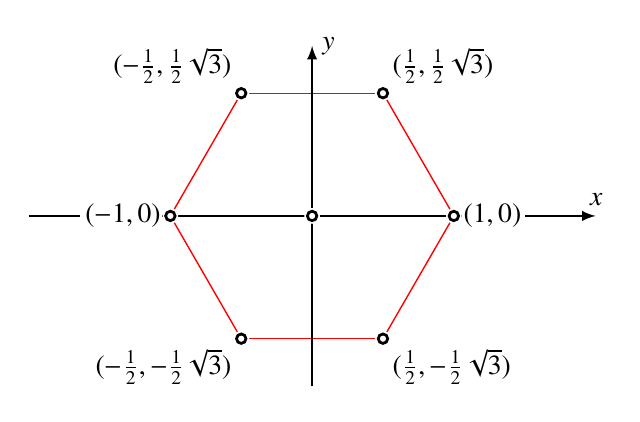
\begin{tikzpicture}[>=latex]

\def\a{1.8}

\def\punkt#1#2{
        \fill[color=white] ({#1},{#2}) circle[radius=0.1];
        \draw[line width=1pt] ({#1},{#2}) circle[radius=0.06];
}

\foreach \p in {0,60,...,300}{
        \draw[line width=0.5pt,color=red] ({\a*cos(\p)},{\a*sin(\p)})--
                ({\a*cos(\p+60)},{\a*sin(\p+60)});
}

\draw[->,line width=0.7pt] ({-2*\a},0)--({2*\a},0)
	coordinate[label={$x$}];
\draw[->,line width=0.7pt] (0,{-1.2*\a})--(0,{1.2*\a})
	coordinate[label={right:$y$}];

\fill[color=white] ({-\a-1.15},-0.2) rectangle ({-\a-0.1},0.2);
\fill[color=white] ({\a+0.1},-0.2) rectangle ({\a+0.9},0.2);

\foreach \p in {0,60,...,300}{
	\punkt{\a*cos(\p)}{\a*sin(\p)}
}
\punkt{0}{0}

%\node at (0,0) [above right] {$0$};
\node at ({\a},0) [right] {$(1,0)$};
\node at ({-\a},0) [left]{$(-1,0)$};
\node at ({0.5*\a},{\a*sqrt(3)/2}) [above right]
	{$\textstyle( \frac12,\frac12\sqrt{3})$};
\node at ({0.5*\a},{-\a*sqrt(3)/2}) [below right]
	{$\textstyle( \frac12,-\frac12\sqrt{3})$};
\node at ({-0.5*\a},{\a*sqrt(3)/2}) [above left]
	{$\textstyle (-\frac12,\frac12\sqrt{3})$};
\node at ({-0.5*\a},{-\a*sqrt(3)/2}) [below left]
	{$\textstyle(-\frac12,-\frac12\sqrt{3})$};

\end{tikzpicture}
\end{document}

